\section{Теоретико-множественные операции}

\begin{definition}[Перечисление множеств]
    Перечислением множеств $A$ и $B$ называется множество, обозначаемое как $A \cap B$, состоящее из тех и только тех элементов, 
    которые принадлежат обоим множествам одновременно. \\ 

    $A \cap B = \left\{ x \mid x \in A \land x \in B \right\}$

    \begin{center}
        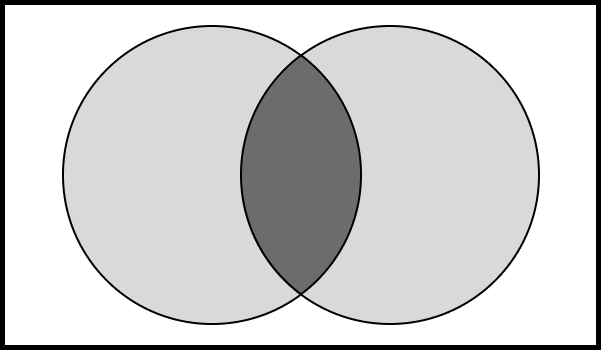
\includegraphics[width=0.25\textwidth]{tex/chapter_2/assets/Intersection.png}\\
    \end{center}
\end{definition}

\begin{definition}[Объединение множеств]
    Объединением множеств $A$ и $B$ называется множество, обозначаемое как $A \cup B$, состоящее из тех и только тех элементов, 
    которые принадлежат хотя бы одному из двух множеств. \\ 

    $A \cup B = \left\{ x \mid x \in A \lor x \in B \right\}$

    \begin{center}
        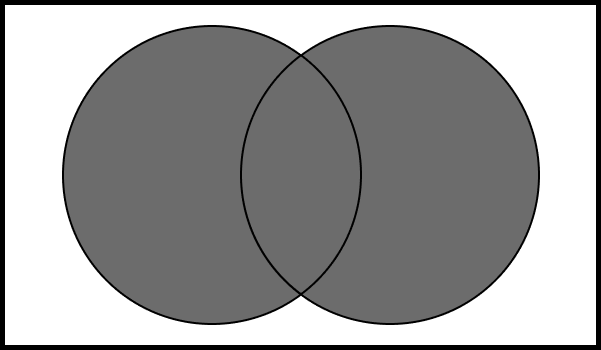
\includegraphics[width=0.25\textwidth]{tex/chapter_2/assets/Union.png}\\
    \end{center}
\end{definition}

\begin{definition}[Теоретико-множественная разность]
    Теоретико-множественной разностью множеств $A$ и $B$ называется множество, обозначаемое как $A \backslash B$, состоящее из тех и только тех элементов 
    множества $A$, которые не принадлежат множеству $B$. \\ 

    $A \backslash B = \left\{ x \mid x \in A \land x \notin B \right\}$

    \begin{center}
        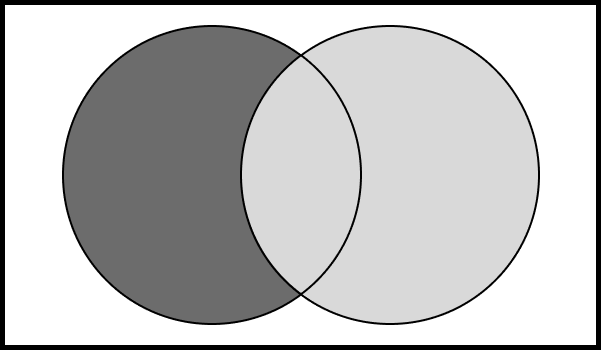
\includegraphics[width=0.25\textwidth]{tex/chapter_2/assets/Subtraction.png}\\
    \end{center}
\end{definition}

\newpage